\chapter{State of the art}
\label{chap:background}

\ac{TTCN-3} is an internationally standardized language
specifically designed for testing and certification.
It has been developed and is maintained by \ac{ETSI},
as well as by leading experts from industry and academia.
This technology has successfully been applied in industry for over a decade
and has proved to work in large industrial tests.

The language provides specific concepts such as
\emph{data matching} (using a powerful template mechanism),
\emph{concurrent execution} of test components
and constructs for handling several alternatives (including timeouts).
The rich type system provides native support for
lists, test verdicts, test system components and timers.
The syntax allows for both \emph{message oriented}
and \emph{procedure oriented} communication.

In order to achieve a high quality of testing,
testcases must be written using a precise notation.
If a testcase (or its purpose) are ambiguous,
they might be subject to interpretation
(which is unacceptable in certification or protocol conformance tests).
The \ac{TTCN-3} language is standardized
and the meaning of each language element is clearly specified.
This leads to independence from particular tool vendors,
since a test case should be executed by every tool in the same way.

Besides the standard textual format used to specify test cases
and record the results of a test execution,
\ac{TTCN-3} provides a graphical format for test specification and execution.


\section{Testcase Examples}

To illustrate the syntax and usage of \ac{TTCN-3}
we will use two example testcases from \citep{ttcn3intro}.
They will show some of the powerful type semantics of the language
and the basic syntax used for communication.

Test code is structured in modules which contain:
\begin{itemize}
\item definitions for data types and testcase behavior
\item an optional control part defining the tests which are to be executed
and their order
\end{itemize}


\subsection{Message oriented example}

The first example will test a \ac{DNS} server.
At first, a simple scenario --- with only one client and one server ---
will be considered.
For the purpose of this example
the structure of \ac{DNS} messages will be simplified as follows:
every message is either a \emph{question} or an \emph{answer}
and has an identification field.
The \verb=DNSMessage= type in Listing \ref{prog:dns-message}
is a \ac{TTCN-3} \verb=record=.
Records are used for defining ordered structured types.
The \verb=messageKind= field has been created as an \verb=enumerated= type
and the \verb=question= and \verb=answer= fields are of type \verb=charstring=.
The \verb=answer= field is optional as it is not present in \ac{DNS} questions.

\begin{program}
\verbatimtabinput{./ttcn3/dns-message.ttcn3}
\caption{DNS message type definition\label{prog:dns-message}}
\end{program}

The actual messages exchanged are instances
of the \verb=DNSMessage= type defined in Listing \ref{prog:dns-message}.
\ac{TTCN-3} uses \verb=template=s to represent either a single instance
or a set of instances of a type.
The ability to represent a set of instances as one template
is a powerful feature of the language.
Thus when defining a template we may use \emph{specific values} but also
\emph{ranges}, \emph{lists} and \emph{matching mechanisms}.
This way received data is automatically checked
to conform to the restrictions imposed on a \emph{receive template}.
If all restrictions are met,
a \emph{match} occurs and the receive operation is successful.
Two templates for \ac{DNS} questions and answers
are defined in Listing \ref{prog:dns-msg-template}.

\begin{program}
\verbatimtabinput{./ttcn3/dns-msg-template.ttcn3}
\caption{Message template definitions\label{prog:dns-msg-template}}
\end{program}

The \verb=ident= field is unique for each question
and allows the mapping of incoming answers to previously issued questions.
This is useful if several requests have been sent
before their respective answers are received.
The \verb=messageType= is fixed for each template
and the \verb=answer= field is omitted in question messages.

After defining message types and templates
it is time to write test cases in which different entities
send and receive messages and set \emph{test verdicts}.
\ac{TTCN-3} models the entities as \emph{components}
which communicate through \emph{ports}.
Ports are seen as infinite queues
which store received messages (or calls) in a \ac{FIFO} manner.
A received message must be processed (and thus removed from the queue)
before subsequent ones can be accessed.
A port type and a component type are defined in
Listing \ref{prog:dns-port-comp}.

\begin{program}
\verbatimtabinput{./ttcn3/dns-port-comp.ttcn3}
\caption{Port and component type definitions\label{prog:dns-port-comp}}
\end{program}

A \ac{TTCN-3} \verb=receive= statement is blocking
until a message corresponding to the expected template is received.
Using a single \verb=receive= statement would block execution forever
if no reply is received or if the first received message is unexpected
(because the ports act as \ac{FIFO} queues
and only the first element can be examined).

\paragraph{The \texttt{alt} statement} is a powerful construct of the language,
allowing the programmer to express several \emph{alternative execution paths}.
An \verb=alt= statement blocks until any one of its alternatives matches.
At every event which may trigger the matching of an alternative
(such as the receiving of a message or the timeout of a timer)
the current state of the system is frozen
and all alternatives are examined in order.
The first alternative that matches is executed
and afterwards control flow moves past the \verb=alt= statement.

The simple testcase in Listing \ref{prog:dns-testcase}
sends a question and defines alternative behavior for:
\begin{itemize}
\item receiving the correct reply
\item receiving an incorrect reply
\item receiving no reply from the name server.
\end{itemize}
The test system will play the role of a \ac{DNS} client
and will test the behavior of a \ac{DNS} server.
The \ac{TTCN-3} system architecture permits the modeling of several entities
by using parallel test components.

\begin{program}
\verbatimtabinput{./ttcn3/dns-testcase.ttcn3}
\caption{DNS example testcase\label{prog:dns-testcase}}
\end{program}


\subsection{Procedure Oriented Example}

This example will show
how \emph{procedure oriented} communication is handled in \ac{TTCN-3}.
The previous \ac{DNS} example will be extended
by assuming that the server has a configuration interface.
Calls to this interface may be made
in order to \emph{add}, \emph{delete} or \emph{change} name server entries.
This may be desirable for initializing the server to a predefined state
before starting any testcases
and also for controlling the name server during the testing process.

We will first define \ac{TTCN-3} signatures
corresponding to the procedures which may be called on the server.
The signatures specify the number and type of \emph{parameters},
the \emph{return value}
and any \emph{exceptions} which may be thrown by the procedure.
The three available signatures are defined in Listing \ref{prog:dns2-sign}
together with a port type.
For this example the port is of \emph{procedure} type.
The keyword \verb=out= specifies that the signatures are ``outgoing'',
meaning that only the test system may invoke them on the \ac{SUT}.

\begin{program}
\verbatimtabinput{./ttcn3/dns2-signatures.ttcn3}
\caption{Signature definitions\label{prog:dns2-sign}}
\end{program}

In the previous (message based) example a structured message type
and two templates (for sending and receiving) have been defined.
In order to call signatures, \emph{signature templates} need to be defined
in a similar manner.
Instead of referring to a type and its fields
the templates now refer to a signature and its parameters.
A template for the \verb=AddEntry= signature is defined
in Listing \ref{prog:dns2-sign-templ}.

\begin{program}
\verbatimtabinput{./ttcn3/dns2-sign-templ.ttcn3}
\caption{Signature template definitions\label{prog:dns2-sign-templ}}
\end{program}

After defining the signatures and signature templates,
a testcase issuing calls to these procedures may be written.
In order to put the tested server in a defined state,
a call to \verb=ClearTable= may be issued at the start of a testcase
followed by several calls to the \verb=AddEntry= procedure.
This way the server's mapping table can be initialized
with a set of known values.

Listing \ref{prog:dns2-call} contains a function
used for calling the \verb=ClearTable= signature
and treating several alternatives.
This signature has no parameters and returns a \verb=boolean= value
representing the success or failure of the call.
The function from Listing \ref{prog:dns2-call} returns
the result of the procedure call
or \verb=false= if no reply was received within a specified timeout period.

\begin{program}
\verbatimtabinput{./ttcn3/dns2-call.ttcn3}
\caption{Procedure call example\label{prog:dns2-call}}
\end{program}

Several alternatives can be specified after the function call.
In this example only return values and timeouts have been checked for.
Besides parameters and return values, a \ac{TTCN-3} signature may also specify
several types of thrown exceptions.
Catching such exceptions may also be specified
as one of the alternatives following the signature call.
In addition to the return value,
a procedure may also return information to the caller
through its \verb=out= or \verb=inout= parameters.


\section{Parallel components and graphical formats}

\ac{TTCN-3} is well suited for testing complex scenarios
where many different entities are running in parallel
and interact asynchronously.
These entities are modeled as \emph{parallel test components}.
The test system can replace one or several components in such a scenario
and incorporate predefined behavior.
Using this approach, all the entities in a large system may be tested
by simulating (replacing) a different set of them for each test case.
An illustration of such a system is provided in
Figure \ref{fig:concurrent-components}
taken from \citep{ttcn3-uc-2007-managing-concurrency}
and available online at \citep{website:ttcn3.org}.%
\footnote{\url{http://www.ttcn-3.org/CoursesAndTutorials.htm}}

\begin{figure}[htb]
\centering
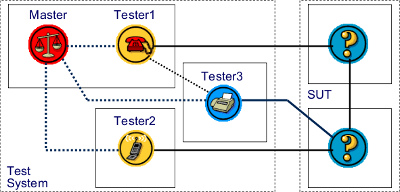
\includegraphics{concurrent-components}
\caption{Testing a large system by replacing a set of its components%
	\label{fig:concurrent-components}}
\end{figure}

This particular representation uses a \emph{\acl{MTC}}
for coordinating the 3 other components simulated by the test system
(\emph{Tester 1--3})
and tests the behavior of 2 entities in the \emph{\acl{SUT}}.
Test system components may be connected to each other
and may also be connected to the \ac{SUT} (using several ports).
The connection with the \ac{SUT} is accomplished by mapping component ports
to ports at the \emph{\acl{TSI}}.
The \ac{TSI} ports are then connected to the real-world \ac{SUT} ports.
Messages are transmitted (and translated between the \ac{TTCN-3} representation
and the real world bits and bytes)
by two components of a \ac{TTCN-3} test system: the codec and port plugin,
as described in section \ref{sec:test-system-arch}.

\ac{TTCN-3} defines a \emph{graphical format} used to represent testcases.
It is equivalent to the \emph{textual format}
used when writing test source code,
but may be easier to understand and more intuitive in some scenarios.

An example of a test representation in the graphical format
is shown in Figure \ref{fig:graphical-test-specification}
taken from \citep{etsi-ttcn3-tutorial}.
The equivalent textual representation of that testcase
is presented in Listing \ref{prog:textual-test-specification}.
The example shows a test for a \emph{DNS} server.
First, the variable (timer) definition is represented.
Then a message send operation and the starting of the timer are shown.
Below them is a representation of the \verb=alt= statement from
Listing \ref{prog:textual-test-specification} with alternatives for
receiving the correct answer, receiving any other answer
and the absence of a response message (a timeout).
The last element represented
is the stopping of the timer at the end of the testcase.

\begin{figure}
\centering
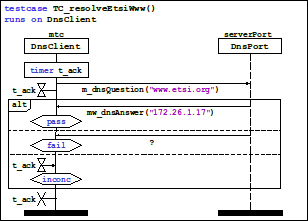
\includegraphics{graphical-test-specification}
\caption{Graphical format of a test specification%
	\label{fig:graphical-test-specification}}
\end{figure}

\begin{program}
\verbatimtabinput{./ttcn3/textual-test-specification.ttcn3}
\caption{Textual format of a test specification%
	\label{prog:textual-test-specification}}
\end{program}

Similar to testcase specifications,
test runs may also be viewed in a graphical format.
Graphical representations of test executions
are an important tool for understanding and analyzing their results.
This form of presentation shows detailed information about:
\begin{itemize}
\item parallel test components active during a testcase execution
\item messages sent and received (including the ports used) and timer events
\item all attempts at matching received data to expected templates
(inside \verb=alt= statements)
\end{itemize}

The same symbols are used as for testcase specification,
but now only the execution path taken is presented
(and not all alternatives in the source code).
%An example of a graphical representation of a test run is shown in
%Figure \ref{fig:graphical-test-execution}.
%It illustrates a simple (successful) protocol test
%involving two test components:
%one of them sends a message and the other returns an expected reply.
The usage of timers and the matching (and mismatching) of alternatives
are also shown in this format.

%\begin{figure}
%\centering
%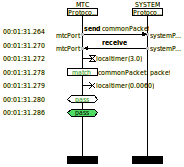
\includegraphics{graphical-test-execution}
%\caption{Graphical format of a test execution%
%	\label{fig:graphical-test-execution}}
%\end{figure}


\section{TTCN-3 Test System Architecture}
\label{sec:test-system-arch}

The previous code examples can be put together
to form a collection of simple tests
called an \emph{abstract test suite}.
It is \emph{abstract}
because a high-level view of the tests to be performed has been defined
but no details about performing the tests in practice have been given.
The communication primitives we have used (e.g.\ \verb=send=, \verb=receive=)
give a conceptual overview of what is going to be tested,
but do not handle the details of encoding and transporting those messages.
In order to run tests in the real world
a translation needs to be made from the abstract specification.

The \ac{TTCN-3} code needs to be compiled to an executable form.
Then some additional information needs to be provided in order to run the tests
against a real \ac{SUT}.
The architecture of a \ac{TTCN-3} test system is shown
in Figure \ref{fig:ttcn3-arch}.
The rest of this section details the most important components.

\begin{figure}
\centering
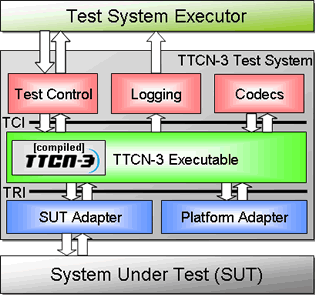
\includegraphics{ttcn3-arch}
\caption{TTCN-3 Test System Architecture\label{fig:ttcn3-arch}}
\end{figure}

\begin{description}
\item[Codecs]
	handle the task of
	encoding outgoing messages to a form understood by the \ac{SUT}
	and decoding received messages
	to their corresponding \ac{TTCN-3} data structures.
\item[\ac{SUT} adapter]
	is another part of the translation layer
	between the abstract test suites
	and the communication with the real \ac{SUT}.
	\ac{TTCN-3} components exchange messages during a testcase by issuing
	(\emph{message oriented} or \emph{procedure oriented})
	operations on ports (e.g.\ \verb=serverPort.send(a_template)=).
	The mappings from abstract ports to their meaning in the real world
	and from abstract communication mechanisms
	to those used by the \ac{SUT}
	are handled by the \ac{SUT} adapter.
\item[Platform Adapter]
	Several functionalities used by a testcase (such as timers)
	are not part of the actual communication method used
	and must be provided by the platform where the test system is running.
	Timers are useful for detecting the absence of messages
	and are implemented in a platform specific manner
	(in addition,
	different testing scenarios may have different timer requirements).
	\ac{TTCN-3} external functions are also platform specific
	and must be provided by this layer.
\item[Test management]
	The language syntax allows test developers to write a control part
	specifying the order of test case execution.
	This solution is adequate for situations
	where test order does not change.
	To allow changes in test execution
	without requiring long re-compilations,
	\emph{Test management} provides support for creating test campaigns.
\end{description}

Two standardized interfaces
specify how the components of a test system fit together.
The \ac{TRI} interface specifies a set of functions
used to abstract communication and timers
from the specific \ac{SUT} and execution environment.
The \ac{TCI} interface is concerned with
test management, logging, encoders and decoders.
It has several sub-interfaces:
\begin{description}
\item[Test management interface]
	(TCI-TM) controls the creation and execution of tests
\item[Coding/Decoding interface]
	(TCI-CD) allows external codecs to be specified when running testcases.
\item[Component Handling interface]
	(TCI-CH) allows the specification of how
	components are created and implemented when deploying the test system
\end{description}
